\documentclass[12pt,a4paper]{article}	%es gibt noch andere Arten of course, wie book zB, aber mit article kommst du gut hin
\usepackage[utf8]{inputenc}
\usepackage[german, english]{babel} 
\usepackage[T1]{fontenc}
\usepackage{amsmath}
\usepackage{bm}
\usepackage{mathtools}

\usepackage{amsfonts}
\usepackage{amssymb}
\usepackage{makeidx}
%\usepackage{esvect}
\usepackage{hyperref}
\usepackage{amsmath}
\usepackage{listings}
\usepackage{subfigure}		%nützlich, wenn du mehrere Bilder in eine Bildumgebung packen möchtest
\usepackage{tabularx}		%für tabellen
\usepackage{chngcntr}
\counterwithin{equation}{section}	%damit Gleichung pro section durchgezählt werden und nicht insgesamt
\counterwithin{figure}{section}		%das gleiche für Bilder
\usepackage{graphicx}
%\usepackage{stackengine}
\usepackage[left=3cm,right=3cm,top=3cm,bottom=3cm]{geometry}
\usepackage[singlespacing]{setspace}	%macht einziligen Zeilenabstand. ansonsten onehalfspacing oder doublespacing

\newcommand{\etan}{\eta_{0}}
\newcommand{\R}{\vv{R}=X\vv{e_{x}}+Y\vv{e_{y}}}
\newcommand{\phid}{\dot{\phi}}
\newcommand{\Yd}{\dot{Y}}
\newcommand{\Xd}{\dot{X}}
\newcommand{\F}{\mathcal{F}}
\newcommand{\p}{\mathcal{P}}
\newcommand{\x}{\textbf}
\newcommand{\norm}[1]{\left\lVert#1\right\rVert}
\newcommand{\abs}[1]{\left\lvert#1\right\rvert}

\begin{document}
\setcounter{section}{2}

\setlength{\parindent}{0pt}


\thispagestyle{empty}

\begin{titlepage}
	\centering
	
\includegraphics[width=0.45\textwidth]{logo_sw.jpg}\par\vspace{1cm}
	\vspace{1cm}
%	{\scshape\Large Spezialisierung\par}
	\vspace{1.5cm}
%	{\LARGE\bfseries working title\\wedge confinement in LC systems  \par}
	{\LARGE\bfseries Assignment Sheet Nr. 3\\  \par}
	\vspace{1cm}
	
	{\large	Paul Monderkamp, Matr.Nr. 2321677\par}
	\vfill
	

	\vfill

% Bottom of the page
	{\large  monderkamp@thphy.uni-duesseldorf.de \par}
	\vspace{2cm}
	%{\large Abgabedatum: 00.04.2017 \par}
\end{titlepage}

\thispagestyle{empty} %macht dass da keine Seitennummer drauf ist.
\newpage	%beendet die Seite und macht auf der nächsten weiter

%\section*{Abstract}
%
%The aim of this specialization report is to summarize the fundamental concepts that are necessary to understand the physical properties of liquid crystal systems and their formation.\\
%The final objective for the masters thesis is to investigate the phase behaviour of those systems in confined space. As a step towards this goal, the algorithm that is used for this problem is introduced and explained. To verify its validity one section of this report is dedicated to recreation of phase behaviour predicted by previous publications on the subject of liquid crystals such as those in this report.\\
%The derivation of the algorithm that is used to generate the corresponding results uses geometrical concepts to guarantee meaningful predictions about the relative positions of the molecules that make up the systems in this thesis. \\
%Beyond that all results are generated via numerical methods. The programming languages used in this thesis are \x{C}/\x{C++} for the generation of the numerical results and \x{MatLab} for the evaluation, processing and visualization of the data. 

%The aim of this bachelors thesis is to provide an overview over the most fundamental theoretical principles which form the basis for the \x{Theory of viscotaxis of microswimmers}. Exemplary geometries of swimming particles are chosen that successively illustrate phenomena typical of the behaviour of systems under the influence of this theory.\\
%Every section which deals with the investigation of a single statement of a problem is divided into two subsections. The first section gives the equations of motion and the respective solutions, and the second one explains the solutions in a physical context and discusses the implications. \\
%All results are purely achieved by analytical methods presented in the respective sections. 

%\newpage
\tableofcontents %macht ein Inhaltsverzeichnis #magic.
\thispagestyle{empty}
\newpage


\section{Exercise 3.1}
\subsection*{Exercise 3.1 (a)}

\begin{figure}[h!]		
\centering
{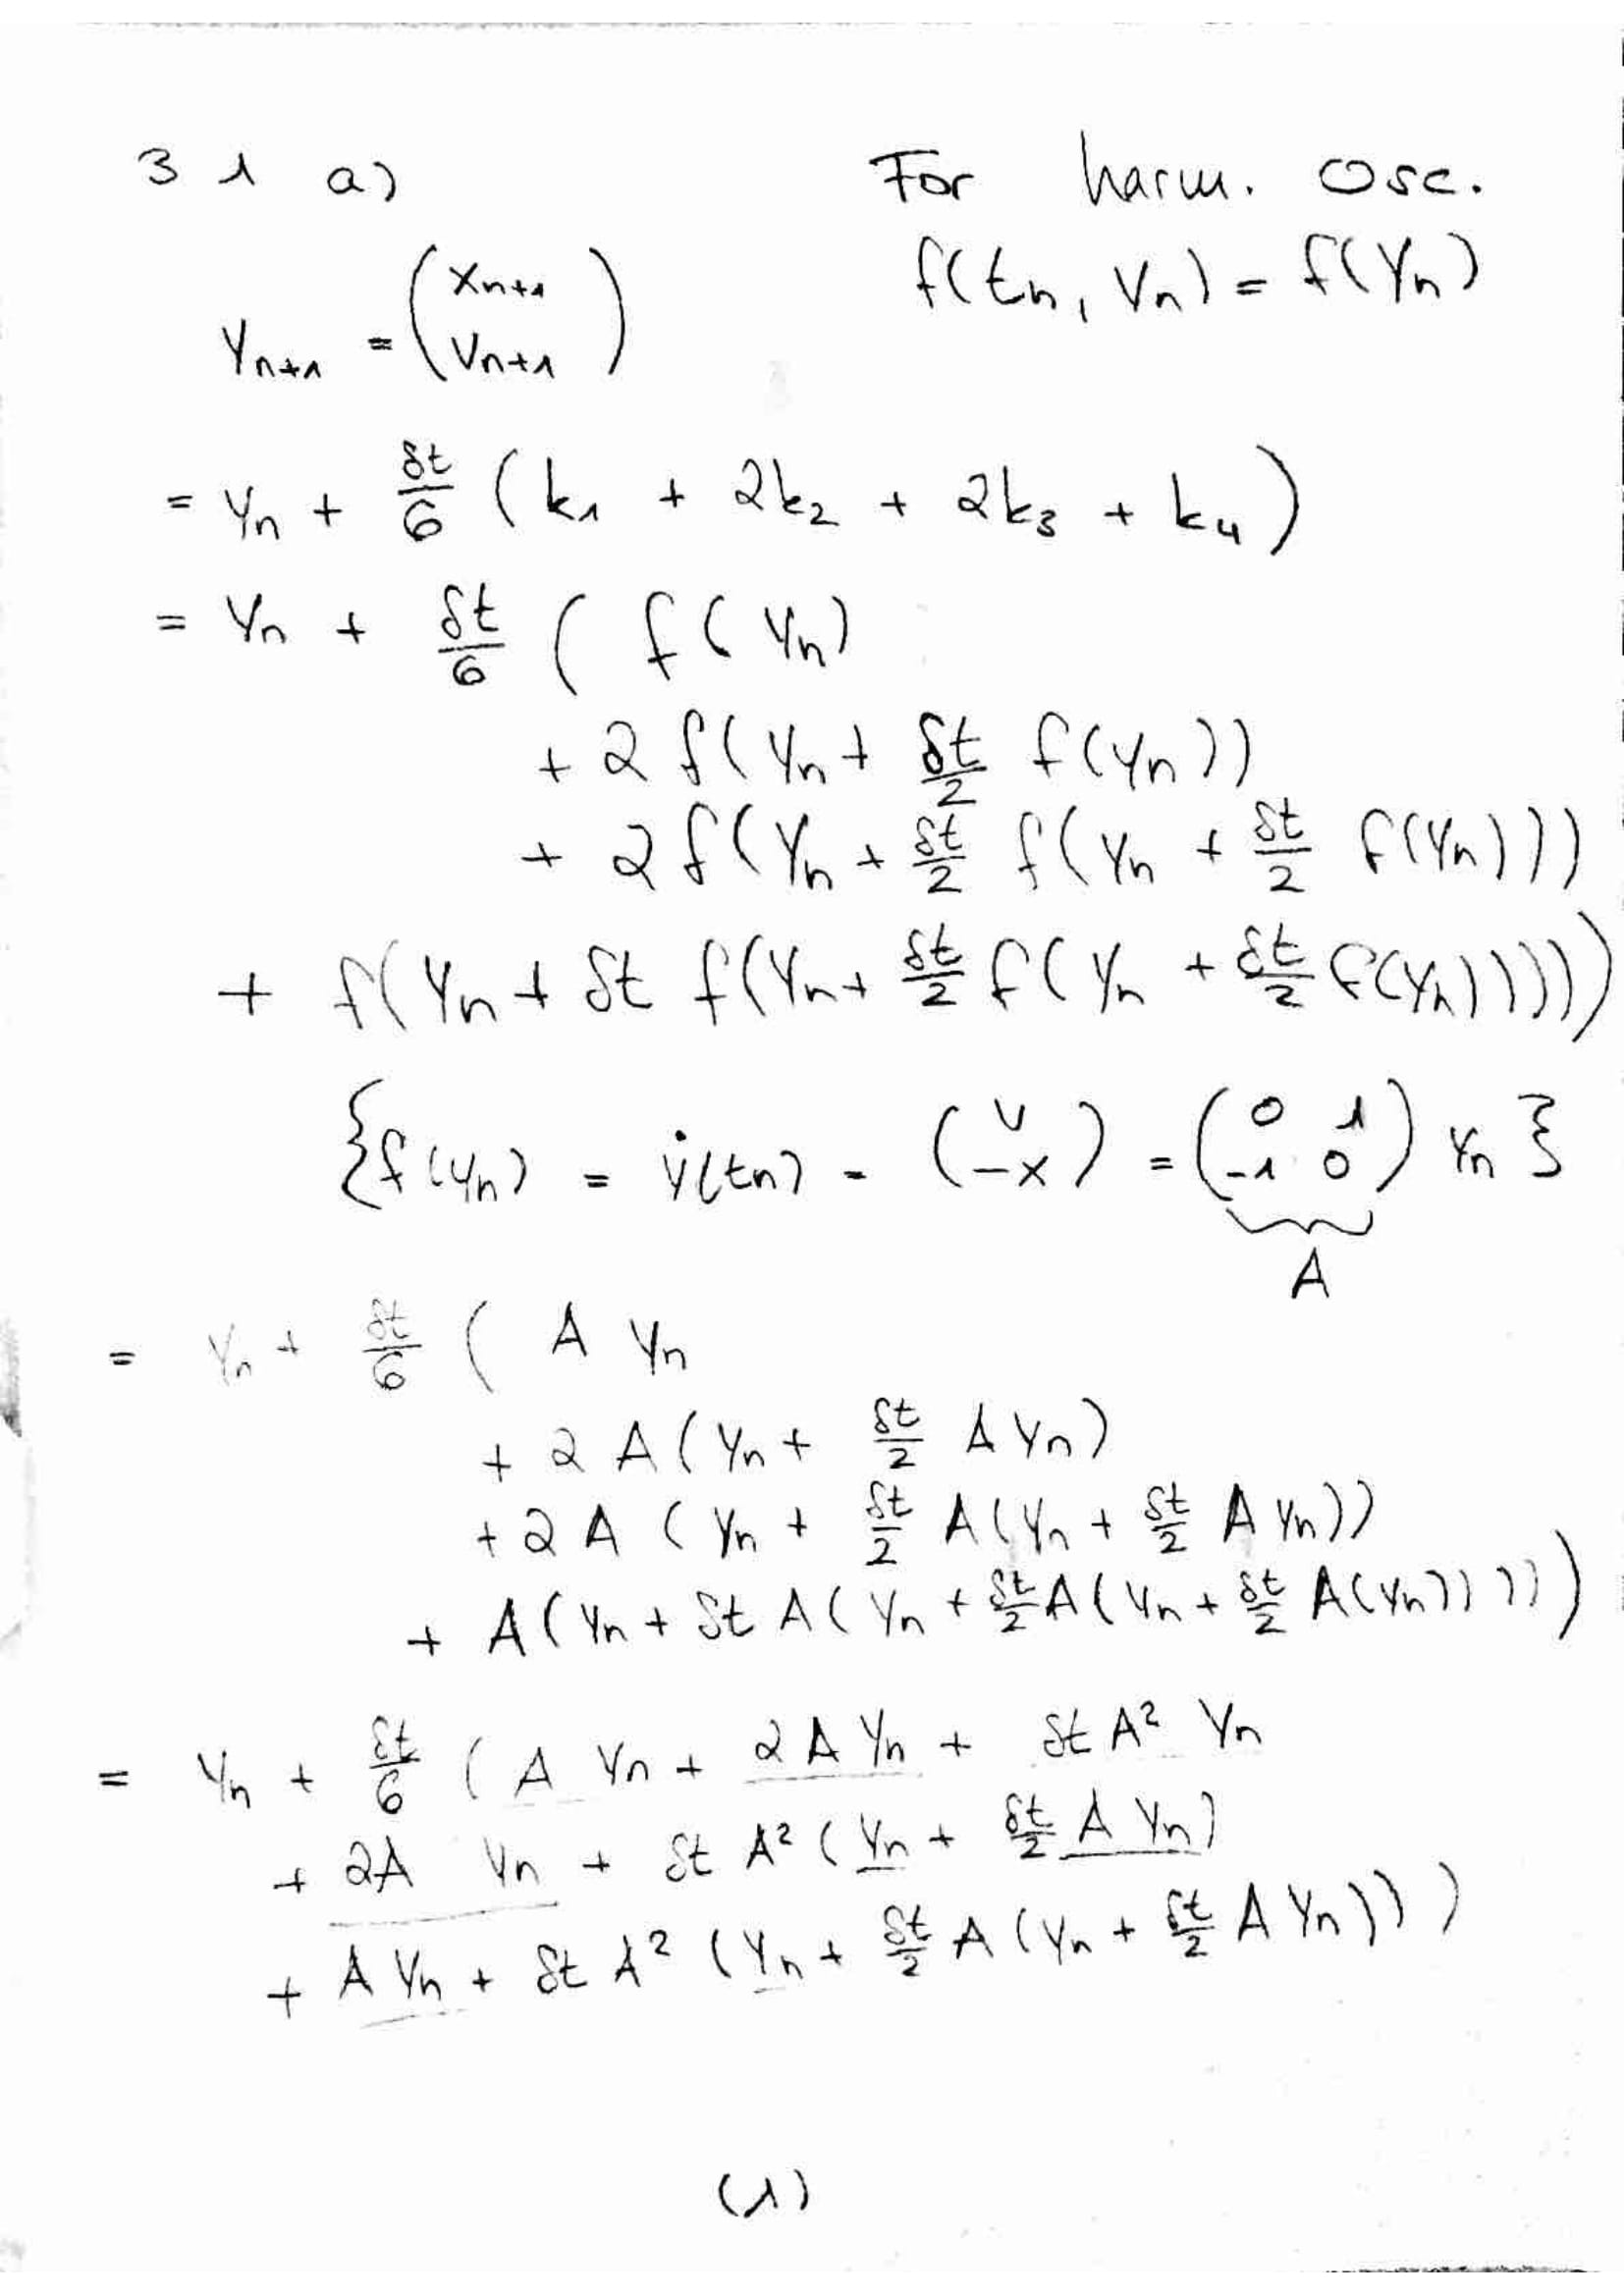
\includegraphics[width=0.8\textwidth]{3_1_a1.jpg}}		
\caption{first part of the derivation of the formula}
\end{figure}

\newpage

\begin{figure}[h!]		
\centering
{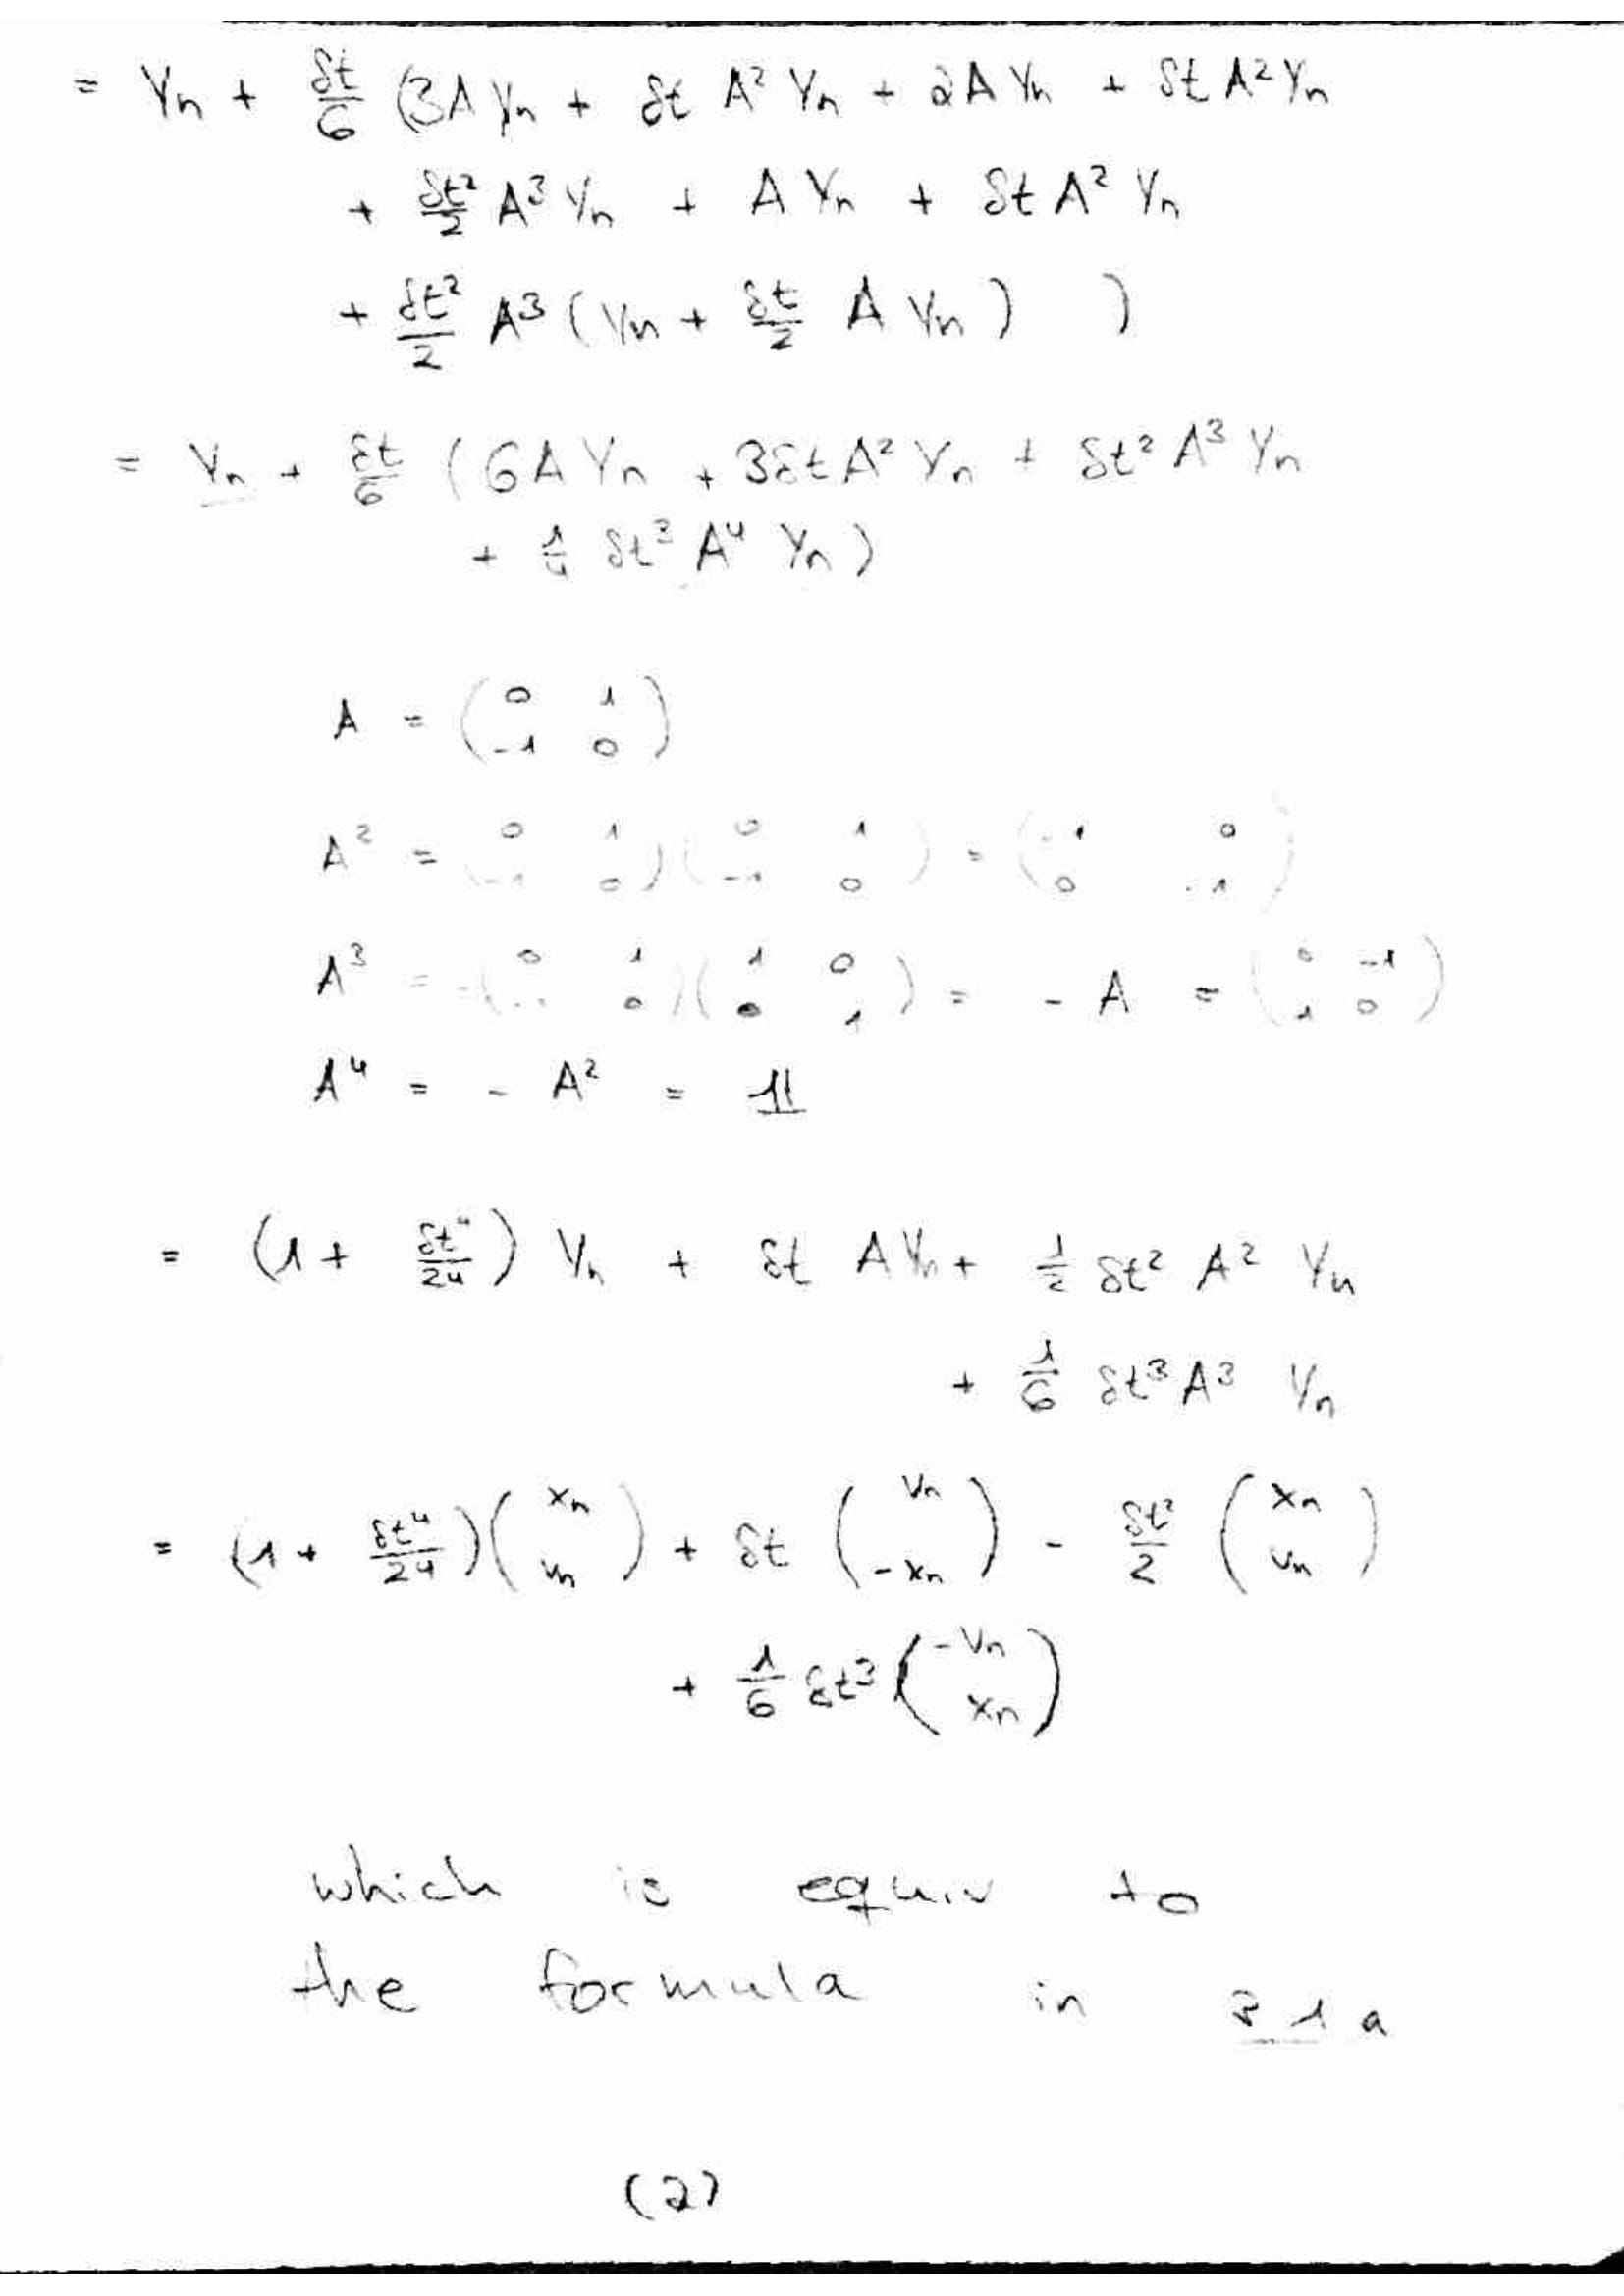
\includegraphics[width=0.8\textwidth]{3_1_a2.jpg}}		
\caption{second part of the derivation of the formula}
\end{figure}

\newpage



\subsection*{Exercise 3.1 (b)}
\subsubsection*{Code}
\lstinputlisting[language=c++]{3_1_b_main.cpp}
%\lstinputlisting{3_1_b_main.cpp}
\newpage

\subsubsection*{Results}
The following results are achived via the code in the previous subsection. 
\begin{figure}[h!]		
\centering
{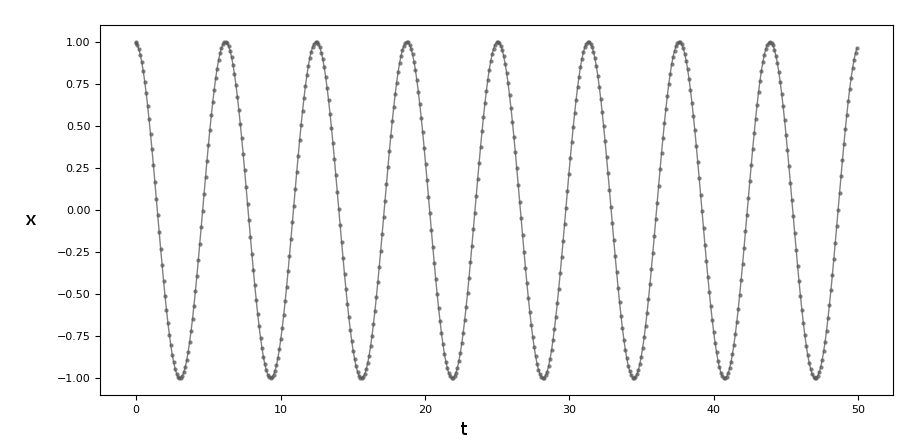
\includegraphics[width=1.0\textwidth]{1bx.png}}		
\caption{time evolution of the x coordinate of the harmonic oscillator}
\end{figure}

Figure 3.3 shows the time evolution of the x coordinate of a one dimensional harmonic oscillator solved with the Runge-Kutta 4 scheme. There is no apparent divergence from the analytical solution visible in the timeframe of the simulation.



\begin{figure}[h!]		
\centering
{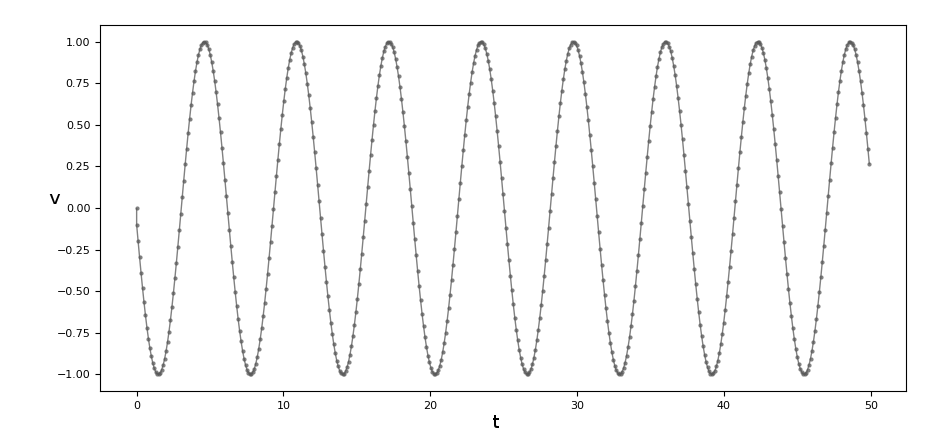
\includegraphics[width=1.0\textwidth]{1bv.png}}		
\caption{time evolution of the velocity of the harmonic oscillator}
\end{figure}

Figure 3.4 shows the time evolution of the velocity of a one dimensional harmonic oscillator solved with the Runge-Kutta 4 scheme. Similarly to the x coordinate, there is no visible instability in the timeframe of the simulation period. 

\newpage

\begin{figure}[h!]		
\centering
{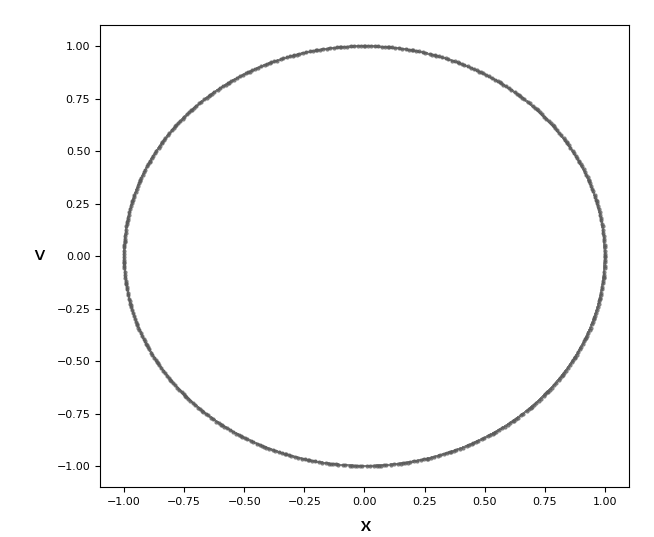
\includegraphics[width=0.5\textwidth]{1bphasespace.png}}		
\caption{phase space trajectory of the harmonic oscillator}
\end{figure}

Figure 3.5 shows the phase space profile for the simulation results above. The trajectory seems reasonably spherical. 

%The two degrees of freedom for a constant number of particles that dictate the phase behaviour are in this case the volume fraction which is proportional to the density and the aspect ratio $p$.\\
%
%
%
%Figure 1.3 shows the phase diagram for for the correspoding liquid crystal 
%as a \\ function of the reduced packing fraction $\rho*$ \footnote{ which is the packing fraction relative to close packing $\rho* = \frac{\rho}{\rho_{cp}}$ } and $\log(p)$.
%
%%\footnote{which is the packing fraction relative to close packing $\rho* = \frac{\rho}{\rho_{cp}$} and $\log(p)$.\\
%
%
%
%The depicted phases are the three mesophases isotropic, nematic and smectic A as well as the three solid ABC and AAA stacked phases, as well as a plastic crystal phase at densities close to close packing [8].
%The name smectic A refers to a layering pattern where the mean orientation is orthogonal to the layers.\\
%The grey space in the phase diagram refers to regions of coexistence of phases where phase transitions occur.
%
%
%
%%plastic solid oben links 
%
%
%
%\newpage
%
%\begin{figure}[h!]	
%\centering
%{\includegraphics[width=0.7\textwidth]{Phase-diagram-of-hard-spherocylinders-with-L-D-between-0-and-60-In-order-to-give-equal1.png}}		
%\caption{Phase diagram of hard spherocylinders [3] with the phases: 
%isotropic (I), nematic (N), smectic A (Sm), AAA stacked solid, ABC stacked solid and plastic crystal phase (P).}
%\end{figure}
%
%Why is it however that those mesophases develop in the first place? 
%
%%Due to the absence of any interaction such as for instance electromagnetic repulsion the system naturally tends towards the state with the highest entropy, while the entropy is the only deciding factor. [9] \\
%
%Naturally the system tends towards the state with the highest entropy. Due to the absence of any interaction such as for instance electromagnetic repulsion, entropy is the only deciding factor [9].
%
%As visible in eq. 1.1 [10], the entropy of a system reflects the probability of a system to reside in a certain subset of phase space \footnote{or configuration space, as momenta are not taken into account due to a low reynolds number regime and the nature of Monte Carlo algorithms}. The sum index $n$ runs over all microstates that are part of the corresponding subset.
%
%\begin{equation}
%S = - k_B\sum_{n}^{} p_n \ln (p_n)
%\end{equation}
%
%Due to the randomness in the fluctuations \footnote{In nature this is due to Brownian motion/ thermal fluctuation. In the Monte Carlo Algorithm this is realized via the random MC-steps (see section 2)} the system most often resides in the macrostate that has the highest probability. \\
%This subset with the highest probability is naturally the one that occupies the biggest volume in phase space. As every configuration of fluid molecules denotes a point in phase space, the macrostate with the highest probability is the one, where all particles can have the maximum number of configurations, or in other words the state, where any  particle has the biggest space to move around. \\
%
%\newpage
%
%At sufficiently low densities, where there is rarely any contact between the fluid molecules this is isotropic density in the orientations and positions, as any particle can reside at any point in space. \\
%As the density increases the particles collide and the macrostate which offers the highest spacial freedom for any particle are the ones where the particles orient in similar directions, given a high enough aspect ratio. This is called nematic phase behaviour. \\
%Upon further increase of the density the macrostate that offers most spatial freedom for any fluid molecule is the one, where in addition to a nematic ordering, the particles also form layers in space. This space is called smectic phase. \\
%At the highest possible densities, the individual particles lose all freedom to move, and the whole fluid has phase transitions into different solid phases, depending on the aspect ratio. \\
%Below aspect ratios of about 3, there is no smectic or nematic phase behaviour. Instead upon increasing density, the fluid undergoes a phase coexistence between the solid phases and the isotropic liquid. 
%
%\newpage
%
%\subsection*{Aim Of The Masters Thesis}
%
%This thesis focuses on investigating systems in the regime of smectic A liquid crystal behaviour where the whole fluid is confined in a wedge geometry between two planes with a relative angle $\zeta$ (Fig 1.4), where $\zeta$ ranges between  $0$ and $\pi$. The interaction with the planes is such that the fluid molecules are affected by surface anchoring effects, which cause orthogonal orientation close to the wedge walls, and thus smectic layers parallel to the corresponding walls [5]. \\
%The fundamental underlying objective of the research is targeted towards to phase behaviour inside the wedge volume beyond the smectic layers close to the wall, as a function of the parameters that are the density, the aspect ratio and the opening angle $\zeta$ of the wedge.
%
%
%\begin{figure}[h!]	
%\centering
%{\includegraphics[width=0.7\textwidth]{p7k02n200.jpg}}		
%\caption{multi body system of spherocylinders}
%\end{figure}
%
%
%
%%\begin{figure}[h!]	
%%\centering
%%{\includegraphics[width=0.7\textwidth]{Phase-diagram-of-hard-spherocylinders-with-L-D-between-0-and-60-In-order-to-give-equal1.png}}		
%%\caption{Phase-diagram-of-hard-spherocylinders [3] with the phases: 
%%isotropic (I), nematic (N), smectic A (Sm), AAA stacked solid and ABC stacked solid.}
%%\end{figure}
%
%\newpage
%
%\section{Description Of The Algorithm}
%
%\begin{figure}[h!]	
%\centering
%{\includegraphics[width=0.7\textwidth]{sdr_abb1.jpg}}		
%\caption{cross section of two spherocylinders with their respective core line segments.}
%\end{figure}
%
%
%The outer shape of a single spherocylinder can be characterized by a core line segment along the main axis of the geometrical body. In that way, all the points on the outer surface of the body have the distance $\frac{\sigma}{2}$ to the core line. In accordance with the depiction in Fig 1.1 the corresponding length of the line segment is $(p-1)\times \sigma$.\\
%In that way the system of non-overlapping spherocylinders can be modeled by numerous line segments.\\
%\\The whole algorithm follows a basic Monte Carlo scheme where a set number of iterations is executed. In each step of the algorithm a random particle in the system is chosen and randomly linearly displaced and rotated to generate trial configurations.\\
%If the potential energy of the system in the trial configuration is lower than in the configuration before the step, the trial configuration is accepted as new
%% avoid repitition of configuration
% configuration. If the potential energy increases compared to the old configuration, the trial configuration is accepted with the probability given by the Boltzmann factor [2]\\
%\begin{equation}
%\kappa = e^{\frac{\Delta U}{k_B T}}.
%\end{equation}
%\\The two governing interactions in the system are given by firstly the hard interaction of the fluid molecules and secondly the wall anchoring interaction that causes the fluid molecules to orient orthogonally close to the wedge walls.
%
%\newpage
%
%\subsection{The Hard Pair Interaction}
%
%Hard interaction between rigid bodies is defined such that the potential is infinity while they are overlapping, and otherwise zero.
%The liquid molecules being hard spherocylinders necessitates a geometric overlap criterion for the construction of the pair potential.\\
%Figure 2.1 shows that two spherocylinders do not overlap as long as the minimal distance between any pair of points on the opposing line segments is greater than $\sigma$.
%Any line segment is parametrized as 
%
%\begin{equation}
%\vec{a}_k = \vec{a}^{(0)}_k + L_k \vec{a}^{(1)}_k
%\end{equation}
%
%where the scalar parameters $L_k$ lie in the interval $\mathcal{I} =[-\frac{1}{2} (p-1) \sigma,\frac{1}{2} (p-1) \sigma]$.
%Finding the mimimal distance of any pair of points on two different line segments equates to the minimization problem of the function $d = \norm{\vec{a}_i - \vec{a}_j}$ in the two dimensional parameter space under the additional conditions that the pair $(L_i, L_j)$ lies in the square $\mathcal{I}^2$ (see Fig. 2.2).
%
%Or analogously minimizing
%\begin{equation*}
%d^2(L_i,L_j) = \norm{\vec{a}_i - \vec{a}_j}^2 
%\end{equation*}
%
%%\begin{equation}
%%= \norm{a^{(0)}_i}^2+\norm{a^{(0)}_j}^2-2\langle a^{(0)}_i, a^{(0)}_j \rangle .
%%\end{equation}
%\begin{equation}
%= ( \vec{a}^{(0)}_i -  \vec{a}^{(0)}_j+ L_i  \vec{a}^{(1)}_i - L_j   \vec{a}^{(1)}_j)^2
%\end{equation}
%
%If $d^2$ assumed constant this equation corresponds to the implicit formula for an ellipse in the two dimensional parameter space [4] (see Fig. 2.2).
%
%\begin{figure}[h!]	
%\centering
%{\includegraphics[width=0.7\textwidth]{ell1.jpg}}		
%\caption{Ellipses in parameter space.}
%\end{figure}
%%caption und plane quadrants und square
%
%\newpage
%
%All points on one ellipse correspond to all pairs of points in real space on the two lines that have the distance d. To find the shortest distance of the line segments one needs to find the tangent point of the smallest possible ellipse with the square $\mathcal{I}^2$.\\
%It can be easily proven that the principal axes of all possible ellipses form an angle of $\frac{\pi}{4}$ with the coordinate axes of $L_i$, $L_j$ (see Appendix 5.1).\\ The possible orientations of the principle axes divides the coordinate plane of the parameter space into four quadrants, corresponding to a coordinate system rotated by $\frac{\pi}{4}$. \\The position of the centre of the concentric ellipses determines the side of the square $\mathcal{I}^2$ at which the smallest possible ellipse is tangent. This yields an extremal point on the tip of one core line segments. What remains of the whole problem is the minimization of $d^2(L_i,L_j)$ in one parameter, which equates to the minimazation of a quadratic equation. 
%
%%\\maybe show properties of focal points
%
%
%\subsection{Surface Anchoring Interaction}
%The second interaction governing the system is the interaction of the particles with certain walls of the enclosed volume. This is introduced to model anchoring effects that occur close to the interfaces when the molecular liquid comes into contact with other phases [5]. 
%\\ In this thesis the boundary conditions require that the mean orientation of the long axes of the fluid molecules are parallel to the normal vector of the walls with which the molecules interact via surface anchoring or wall anchoring.
%This aims to induce the fluid to form smectic layers close to the wall.\\ 
%The interaction potential that is chosen to model surface anchoring effects has the form of
%\begin{equation}
%\mathcal{V}(\theta,x) = 
%\begin{cases}
%V_0\sin^2(\theta) \exp(-\xi(x-\frac{\sigma p}{2})) & \text{ for }  x > \frac{\sigma p}{2}  \\
%V_0\sin^2(\theta)  & \text{ for }  x < \frac{\sigma p}{2}  \\
%\end{cases}
%\end{equation}
%
%where $\theta$ is the relative angle of the normal vector of the wall (see Fig.2.3), and $x$ is the distance of the geometrical centre (C) of the corresponding fluid molecule to the surface. The constant $V_0$ is of the order of magnitude of about $100$ $k_B T$ and $\xi$ is about $\frac{10}{\sigma}$.\\
%The factor that depends on $\theta$ has minima at $n\pi$, $n \in \mathbb{N}$. 
%\\Due to the fact that the orientation of the spherocylinders at $\theta = 0$ is geometrically equal to the orientation $\theta = \pi$ and the following periodicity it is convenient to reduce the problem to only one minimum at $\theta = 0$.\\
%
%\begin{figure}[h!]	
%\centering
%{\includegraphics[width=0.7\textwidth]{WAcyl.jpg}}		
%\caption{Geometrical length scales of the system close to the walls}
%\end{figure}
%
%
%\newpage
%The underlying Monte Carlo algorithm causes the spherocylinders to fluctuate around this minimum for constant $x$.
%The dependence on $x$ is chosen such that the strength of the  potential as a function of $x$ is independent of $x$ when the geometric centre is closer to the wall than half of the length of the spherocylinder. When the geometric centre is further away from the surface of the wall the strength of the potential is rapidly expoentially decreasing on the length scale of the particles.\\
%This potential causes the particles to orient towards a perpendicular orientation and the exponentially decreasing factor restricts the orientational potential to the first layer at the surface (see Fig. 2.4).
%
%\newpage
%
%%\begin{figure}[h!]	
%%\centering
%%{\includegraphics[width=0.7\textwidth]{WA.png}}		
%%\caption{Surface anchoring effects at low densities}
%%\end{figure}
%
%\begin{figure}[h!]	
%\centering
%{\includegraphics[width=0.9\textwidth]{wand1_2.jpg}}		
%\caption{Surface anchoring effects at low densities}
%\end{figure}
%
%
%
%
%%diagramm erneuern und punkt im phasendiagramm angeben
%Figure 2.4 shows a system of particles that are confined to the $[0,1]^3$-box, and are interacting with the lower wall of the box. 
%It shows how at a point of the phase diagram, where the exptected phase is isotropic due to low density, the molecules prefer perpendicular orientation close to the $z = 0$ plane, while otherwise being unordered. 
%
%
%\newpage
%
%\section{Resulting Phases According To Literature}
%As mentioned in the introduction, this thesis focuses on the investigation of a liquid crystal in the regime of the phase diagram where the expected phase is smectic layering. \\
%In order to be able to investigate the phase behaviour of spatially confined liquid crystal systems, it is useful to show, that the algorithm can reproduce the phases of free unconfined liquid crystal systems as predicted in previous work. 
%%to justify smectic layering without the specific geometrical confinements as well as
%
%Accordingly %reasonable wall anchoring strength in the numerical model, 
%this section aims to reproduce smectic A, nematic and isotropic phase behaviour of unconfined liquid crystals with periodic boundary conditions in the regimes predicted by the phase diagram from Belhuises and Frenkels \textit{Tracing the phase boundaries of hard spherocylinders} [9]. 
%\\
%Future research will include confinement of the fluids, where several surfaces with wall anchoring potentials are present. Thus to tune the parameters of the interactions and show physically reasonable behaviour under the influence of surface anchoring effects with a single wall, this section also includes simulations of corresponding liquid crystal systems .
%%under the presence of an additional wall that causes wall anchoring effects, as well as the original phase behaviour of the free fluid molecules with periodic boundary conditions as depicted in the phase diagram. 
%
%\begin{figure}[h!]	
%\centering
%{\includegraphics[width=0.8\textwidth]{L3kreuz.png}}		
%\caption{cut out of the phase diagram in Fig 1.3 for small aspect ratios [3] with the phases: 
%isotropic (I), nematic (N), smectic A (Sm), AAA stacked solid (S), and plastic crystal phase (P).}
%\end{figure}
%
%\newpage
%
%The red markers in the phase diagram show the points that denote the values for the simulation which sections 3.1 and 3.2 show the results of. \\
%The point in the phase diagram that corresponds to smectic phase behaviour has the coordinates $\rho* = 0.6$ and $\frac{L}{\sigma} = 4.5$. This coincides with an absolute packing fraction of $\rho = 0.52$ and an aspect ratio of $p = 5.5$.\\
%The second point in the phase diagram which corresponds to nematic phase behaviour has the coordinates $\rho* = 0.47$ and $\frac{L}{\sigma} = 5$. This coincides with an absolute packing fraction of $\rho = 0.41$ and an aspect ratio of $p = 6$.\\
%The third point in the phase diagram denotes isotropic phase behaviour where the orientation vectores $\vec{a}^{(1)}_k$ (compare Eq. 2.2) are unitarily distributed on the unit sphere $\mathcal{S}_2$ and the spatial density is homogeneous.
%The corresponding parameters in the phase diagram are $\rho* = 0.4$ and $\frac{L}{\sigma} = 1.0$. This gives an absolute packing fraction of $\rho = 0.33$ and an aspect ratio of $p = 2$.
%
%\newpage 
%\subsection{Isotropic Phase}
%\subsubsection{Unconfined Liquid}
%
%Figure 3.2 shows the cross section of a liquid crystal system with parameters that are predicted to lie within the parameter region of isotropy.  \\
%As described above an isotropic liquid crystal is characterized by the homogeneous density of the positions of the geometrical centres of the particles as well as the absence of a preferred direction of orientation.  This happens at suffiently low densities where the particles are not forced into alignment due to scarcity of space and low aspect ratios, where the individual particles can rotate while interacting with a sufficuently small amount of other particles that disturb the rotation. 
%
%
%\begin{figure}[h!]	
%\centering
%{\includegraphics[width=0.8\textwidth]{isotr.jpg}}		
%\caption{visualization of the simulation results for a liquid crystal in the parameter regime for an isotropic phase behaviour}
%\end{figure}
%
%Accordingly the density and ehe aspect ratio of this particular simulation is given by a greatly smaller number than the values used in the simulation of the nematic and smectic phase. The packing fraction is equal to $\rho = 0.33$ whereas the aspect ratio is equal to  $p = 2$.\\
%
%\newpage
%
%\begin{figure}[h!]	
%\centering
%{\includegraphics[width=0.7\textwidth]{isotrdens.jpg}}		
%\caption{distribution of the particles along the x axis (top, red), distribution of the particles along the y axis (middle, green), and distribution of the particles along the z axis (bottom, blue)}
%\end{figure}
%
%Figure 3.3 shows the density of particles along the different Cartesian axes within the simulation volume.\\
%In the following sections about nematic and smectic phase behaviour the geometry of the simulation is chosen such that the system is isotropic along the x-y plane. In both cases the director points in the direction of the z axis and in the case of the smectic A liquid crystal the layers therefore are along the x-y plane, such that the density only varies along the z axis. This distinguished role of the z-axis suggests a comparison of the densities along the z axis. For the sake of completeness however Figure 3.3 also shows the density along the x and y axis. \\ 
%
%It is visible that the geometric centres of the particles are isotropically distributed in the simulation box. The fine binning of the histograms visualizes the fluctuations whereas a more coarse binning would show of completely identical height. 
%\newpage
%
%
%
%
% 
%
%\begin{figure}[h!]	
%\centering
%{\includegraphics[width=1.0\textwidth]{angledataisotr.jpg}}		
%\caption{distribution of the azimuthal angle $\phi$ (left), distribution of polar angle $\theta$ of the long axes of the particles to the z axis (right)}
%\end{figure}
%
%Figure 3.4 (left) shows the distribution of the azimuthtal angle $\phi$. It is visible that the system shows no preferred direction of orientation in the x-y plane. Therefore $\phi$ is uniformly distributed. \\
%Figure 3.4 (right) shows the corresponding distribution of the polar angle $\theta$.\\
%As visible in figure 3.5 and the description of the nematic order on the following pages the orientation vectors of the particles are distributed uniformly on the unit sphere $S_2$. The shape of the distribution in $\theta$ comes from the fact that the area of the belts with constant $\theta$ scales with $\sin(\theta)$. This leads to a sinusoidal distribution of the polar angle in $\theta$.
%
%\begin{figure}[h!]	
%\centering
%{\includegraphics[width=0.7\textwidth]{S2_isotr.jpg}}		
%\caption{distribution of the orientations of the particles on the unit sphere}
%\end{figure}
%
%\newpage
%
%A more straightforward mathematical method to investigate the nematics i.e. the orientational structuring of the liquid crystal system involves the so called nematic order parameter $\mathcal{Q}$ which is a $3\times3$ tensor that is defined as
%\begin{equation}
%\mathcal{Q} =\frac{1}{2} \left\langle 3 \hat{u}_k \otimes \hat{u}_k -\mathcal{I}_3  \right\rangle_k
%\end{equation}
%where $\mathcal{I}_3$ is the $3\times3$ unit matrix. \\
%%$\left\langle \right\rangle$
%
%This nematic order parameters has the properties that it is traceless such that its three eigenvalues sum up to zero. The largest eigenvalue $\lambda_1 =: \mathcal{S}$ is an index of how strongly a system orients along a certain axis, which is given by the corresponding eigenvalue. The two other lower eigenvalues $\lambda_1, \lambda_2$ indicate whether the system is uniaxial or biaxial expressed in whether the eigenvalues are identical or different. \\
%For example a system where all particles are oriented in one direction would correspond to a tripel of eigenvalues $(1.0, -0.5, -0.5)$ (See Appendix 5.2).
%A system with isotropic nematics as above where the orientations are completely isotropically distributed corresponds to eigenvalues that are all equal to zero. \\
%The tripel of eigenvalues for the simulation above is equal to $(0.04772,  -0.00081, -0.04690)$. The small absolute values of the eigenvalues shows that the system is to a very good approximation indeed nematically isotropic.\\The correspoding eigenvectors are given as
%\begin{equation}
%\begin{pmatrix}
% -0.74012\\
% -0.42367\\
%  0.52222
%\end{pmatrix},
%\begin{pmatrix}
% -0.58595\\
%   0.02524\\
% -0.80995
%\end{pmatrix},
%\begin{pmatrix}
% -0.32997\\
% 0.90546\\
% 0.26693
%\end{pmatrix}.
%\end{equation}
%As the system has no preferred direction of orientation the pricipal axes of the nematic order for this case have no special significance. \\
%
%time evol. \\
%
%compare diff char eq. times\\
%
%very little disturbance, fast eq. investigate eq. times as function of system size \\
%
%\subsubsection{Interaction With Wall}
%
%density as function of z, mean angle as function of z
%
%\newpage
%
%\subsection{Nematic Phase}
%\subsubsection{Unconfined Liquid}
%
%%In the sections about nematic and smectic phase behaviour the geometry of the simulation is chosen such that the system is isotropic along the x-y plane. In both cases the director points in the direction of the z axis and in the case of the smectic A liquid crystal the layers therefore are along the x-y plane, such that the density only varies along the z axis. This distinguished role of the z-axis suggests a comparison of the densities along the z axis. \\ 
%%
%%In sectiom 3.1 about the isotropic phase it is visible that the density along the z axis is homogeneous.
%%hier auch. compare with smectic. 
%
%\subsubsection{Interaction With Wall}
%
%\begin{figure}[h!]	
%\centering
%{\includegraphics[width=1.0\textwidth]{placeholder.jpg}}		
%\caption{aad}
%\end{figure}
%
%make upper wall also interacting
%
%\newpage
%
%\subsection{Smectic Phase}
%
%\subsubsection{Unconfined Liquid}
%
%
%
%\subsubsection{Interaction With Wall}
%
%Figure 3.3 shows the cross section of the layers of a system that obeys the predictions for a smectic liquid crystal system given in the phase diagram in Figure 3.1.\\
%The parameters for the aspect ratio and the absolute volume fraction are as given above $p = 5.5$ and $\rho = 0.52$.
%As it is the main characteristicum for smectic A liquid crystals the positions in space are layered and the orientations of the long axes of the particles are distributed around the normal vector of the layers.\\
%
%\begin{figure}[h!]	
%\centering
%{\includegraphics[width=0.6\textwidth]{placeholder.jpg}}		
%\caption{cross section of the smectic A liquid crystal system along the z-x plane behaviour}
%\end{figure}
%
%\newpage
%
%Figure 3.4 (left) shows a view along the z axis of the system in the equilibrated state. From the structure of the positions in the x-y-plane it is visible, that the positions of the fluid molecules inside the smectic layers are disordered unlike for example in a smectic B liquid crystal, where the positions inside the layers are structured on as triangular lattice. 
%
%%\begin{figure}[h!]	
%%\centering
%%{\includegraphics[width=0.6\textwidth]{topviewsmecticcut.jpg}}		
%%\caption{smectic phase}
%%\end{figure}
%
%\begin{figure}[h!]	
%\centering
%{\includegraphics[width=1.0\textwidth]{placeholder.jpg}}		
%\caption{cross section of the system in Fig. 3.5 along the x-y plane (left), and distribution of angle $\theta$ of the long axes of the particles to the z axis (right)}
%\end{figure}
%
%Figure 3.4 (right) shows the distribution of the angle $\theta$ (see Eq. 2.4) which is the relative angle of the long axes of the fluid molecules to the z axis. As the configuration is chosen such that the positions of the particles layer across planes parallel to the plane $z=0$, this is also the relative angle to those planes, as well as the relative angle to the single wall which causes wall anchoring effects. \\
%
%The polar angle $\theta$ lies within the interval $[0,\pi)$. For convenience and due to the $\pi-$periodicity however this graph shows the distribution centred around 
%$\theta = 0$ to enable the observation of what is in physical reality a single peak.\\
%
%The diagram shows that the orientation of the particles fluctuate around the $\theta = 0$ axis which denotes the director of the fluid. It is also visible, that there is no significant fluctuation beyond a distance of about $0.4$ rad to director orientation. \\
%
%\newpage
%
%The three eigenvalues of the nematic order parameter are $0.99080$, $-0.49492$ and 
%$ -0.49588$. The very good proximity the of the two lower eigenvalues confirms uniaxial nematics as it is exptected in the nematic liquid crystal. 
%The three corresponding eigenvectors are given in equation 3.1. \\
%The first eigenvector denotes the axis of orientation of the director, which is parallel to the unit vector in z direction $\vec{e_z}$ up to a very small margin. 
%
%\begin{equation}
%\begin{pmatrix}
% 0.00227\\
%-0.00690\\
%-0.99997
%\end{pmatrix},
%\begin{pmatrix}
% 0.94354\\
% 0.33127\\
%-0.00015
%\end{pmatrix},
%\begin{pmatrix}
% -0.33126\\
%0.94351\\
%-0.00726
%\end{pmatrix}
%\end{equation}
%
%\newpage
%
%\section{Raute mit waenden aber per.b. in y}
%one angle (pi/4?)\\
%
%ueberarbeite summary/prosp\\
%
%\newpage

%\section{Summary/Prospects}
%As a part of the pre-masters thesis specialization this report summarizes the most important concepts which are essential for the generation of research results as intended in the masters thesis. \\
%\x{Section 1} aims to introduce the concept of a liquid crystal with its mesophases as intermediate state between solid crystals and disordered isotrope fluids. It explains the formation of those phases due to entropy.  Furthermore the fundamental physical objective and research question in formulated.\\
%\x{Section 2} describes the Monte Carlo Algorithm with which the simulation of the fluid is achieved. Both interactions that govern the behaviour of the liquid crystal are explained.\\
%In \x{Section 3} the phases that are introduced in section 1 are reproduced after previous publications. This is achieved with the algorithm that is described in section 2. This is done in order to confirm the physical validity of the procedures of the algorithm, and the ability of the subroutines to produce physically relevant results.\\
%\\
%One of the biggest factors for the fast equilibration of the applied Monte Carlo algorithms in this pre-thesis is, that for the interaction with one surface or the simulation of an unconfined fluid within periodic boundaries all simulation volumes were able to be chosen rectangular. Furthermore the initialization of the positions could be chosen such that all particles fill the volume isotropically.\\ 
%When investigating the physical problem that is described in the \x{Aim Of The Masters Thesis} this is abviously not possible anymore, due to the unisotropic nature of the simulation volume (see Fig 1.4).\\
%\\
%A central problem of further investigation of this physical phenomenon will thus revolve around the determination of an obtimal initialization for the positions and orientations of the fluid molecules to guarantee fast equilibration in the simulation. 

%different angles wedge confinement
%\newpage


%
%\begin{equation}
%\vec{r_{1,2}}=\vec{R}\mp r\begin{pmatrix}
%\cos\phi\\
%\sin\phi
%\end{pmatrix}.
%\end{equation}


 


%\newpage

%\addtocontents{toc}{\protect\newpage}





%\section{Summary/ Prospects}
%
%
%\newpage



%\section{Appendix}
%
%%\subsection{Principle Axes Of Ellipses In The Overlap Criterion}
%%
%%The equation of an ellipse in the coordinate frame of the principle axes has the form 
%%\begin{equation}
%%A x+By-C=0.
%%\end{equation}
%%equation (2.3) has the form 
%%\begin{equation*}
%%(\vec{a}^{(0)}_i -  \vec{a}^{(0)}_j+ L_i  \vec{a}^{(1)}_i - L_j   \vec{a}^{(1)}_j)^2.
%%\end{equation*}
%%The coordinate transformation 
%%\begin{equation*}
%%u = L_i+ L_j,
%%\end{equation*}
%%\begin{equation*}
%%v = L_i- L_j,
%%\end{equation*}
%%is chosen, where the coordinate axes correspond to $\abs{L_i} = \abs{L_j}$, so a rotation about an angle of $\frac{\pi}{4}$.
%%Performing this transformation on equation (2.3), one gets the general shape of (5.1), which shows that the principle axes of the ellipses in section (2.1) form in fact an angle of $\frac{\pi}{4}$ with the coordinate axes $L_i,L_j$.
%
%\newpage

%\subsection{Nematic Order Parameter For Perfect Nematics}
%
%%\begin{figure}[h!]	
%%\centering
%%{\includegraphics[width=0.6\textwidth]{IC.jpg}}		
%%\caption{Liquid crystal in the configuration of perfect nematics}
%%\end{figure}
%
%Figure 5.1 shows a liquid crystal system in the nematic regime for the special configuration where all spherocylindrical fluid molecules are oriented in the same direction. This configuration is used as starting configuration for most of the Monte Carlo simulations. This configuration has perfect nematics in contrast to the system in 3.1.1 where the distribution of orientations is isotropic. \\
%This configuration reflects one extreme of the nematic order parameter where the upper eigenvalue $\mathcal{S}$ is equal to one due to the perfect orientation and the other two eigenvalues are $\lambda_{2,3} = -0,5$ due to tracelessness and uniaxiality. The \x{MatLab} script that calculated the above for all the simulations in this thesis gives the eigenvalues out as (-0.50000,-0.50000,1.00000) and the corresponding eigenvectors as
%
%\begin{equation}
%\begin{pmatrix}
% 1\\
% 0\\
% 0
%\end{pmatrix},
%\begin{pmatrix}
% 0\\
% 1\\
% 0
%\end{pmatrix},
%\begin{pmatrix}
% 0\\
% 0\\
% 1
%\end{pmatrix}
%\end{equation}
%
%which reflects the perfect orientation along the z-axis. 
%
%\newpage

%\section{Acknowledgements}
%
%
%\newpage

%\section{References}
%%\begin{enumerate}
%
%%\item i suppose it would be reasonable to give a justification for the low reynolds number and attach a source. 
%
%%%\item das hier ist ne
%%\item durchnummerierte Aufzählung.
%%\item bietet sich natürlich für die Quellen an.
%%\end{enumerate}
%%Wenn du da noch eckige Klammern drum haben willst:\\
%\renewcommand{\labelenumi}{[\theenumi]}
%\begin{enumerate}
%
%\item item 1
%URL: \\
%\url{url1} \\
%published as: item1, last visited: date


%\end{enumerate}


\newpage

%\section{Statutory Declaration}
%
%I declare that I have developed and written the enclosed thesis completely by
%myself, and have not used sources or means without declaration in the text. Any
%thoughts from others or literal quotations are clearly marked. The thesis was
%not used in the same or in a similar version to achieve an academic grading or is being
%published elsewhere.
%\\
%\\
%\\
%\\
%\underline{\hspace{7cm}}\\
%Date, Paul Monderkamp

\end{document}
